\documentclass[12pt]{article}
\usepackage[top=1cm, bottom=3cm, right=2cm, left=2cm]{geometry}
\usepackage{amsfonts, amssymb, amsmath, hyperref}
\usepackage{graphicx}
\usepackage[T1, T2A]{fontenc}% T2A for Cyrillic font encoding
\usepackage[english, russian]{babel}
\usepackage[justification=centering]{caption}
\usepackage[caption]

\pagestyle{empty}

\begin{document}
\title{\textbf{Лабораторная работа 2.1.6}\\[2pt]{Эффект Джоуля–Томсона}}
\date{\today}
\author{Татаурова Юлия Романовна}

\begin{document}
\maketitle
\textbf{Цель работы: }\\
1) определить изменения температуры углекислого газа 
при протекании через малопроницаемую перегородку при разных начальных 
значениях давления и температуры;\\
2) вычислить по результатам опытов коэффициенты 𝑎 и 𝑏 модели Вандер-Ваальса.\\ \indent
\textbf{Оборудование: }трубка с пористой перегородкой; труба Дьюара; термостат
жидкостной; дифференциальная термопара; вольтметр универсальный (мультиметр);
балластный баллон; манометр.\\ 

\section*{Теоретические сведения}
\indent
\indent{Эффектом Джоуля–Томсона называется изменение температуры газа, медленно
просачивающегося из области высокого в область низкого давления в условиях 
тепловой изоляции. Коэффициентом Джоуля-Томсона называется величина:}
\begin{equation}
    \mu_{\text{д-т}} = \frac{\Delta T}{\Delta P} 
\end{equation} 
Выведем некоторые теоретические соотношения:
$$Q=0 \rightarrow \delta A = -\Delta U \rightarrow P_1 V_1-P_2 V_2 = 
(U_2 + \frac{\mu {\upsilon_2}^2}{2})-(U_1 + \frac{\mu {\upsilon_1}^2}{2})$$\\
Молярная энтальпия: $H = U+PV$, тогда 
$$H_1 - H_2 = \frac{\mu ({\upsilon_2}^2 - {\upsilon_1}^2)}{2}$$ 
Однако кинетическая энергия газа оказывается пренебрежимо малой, поэтому
$$H_1 \approx H_2$$
Рассмотрим реальный газ как газ Ван-дер-Ваальса:
$$\left ( P+\frac{a}{V^2}\right )(V-b) = RT$$
$$U = C_\text{v}T-\frac{a}{V}$$
Тогда энтальпия:
\begin{equation} \label{eq:entalp}
    H = U+PV=C_{\text{v}}T+RT\frac{V}{V-a} - \frac{2a}{V}
\end{equation}
При этом для упрощения вычислений будем считать газ разряженным и 
считать объем по формуле Клайперона-Менделеева $V \approx \frac{RT}{P}$, 
а также с учетом того, что $b \ll V$ из \ref{eq:entalp} получаем:
\begin{equation} \label{eq:entalpy}
H \approx C_{\text{P}}T + P \left (b- \frac{2a}{RT} \right )
\end{equation}
Так же будем считать изменения температуры в опыте небольшим 
$\frac{\Delta T}{T} \ll 1$. Тогда полагая $\Delta H = 0$ из \ref{eq:entalpy}:
\begin{equation}\label{eq:mu}
    \mu_{\text{д-т}} = \frac{\Delta T}{\Delta P} \approx -
    \frac{b - \frac{2a}{RT}}{C_{\text{P}}}
\end{equation}
Из \ref{eq:mu} видно, что существует такая температура (\emph{температура инверсии}),
при которой знак эффекта меняется:
\begin{equation}\label{eq:temperature}
    T_{\text{инв}} = \frac{2a}{Rb}
\end{equation}

\section*{Экспериментальная установка}
Схема установки для исследования эффектов Джоуля-Томсона в углекислом газе 
представлена на ниже.\\
\begin{figure}[h!]\label{fig:setup}
    \centering
    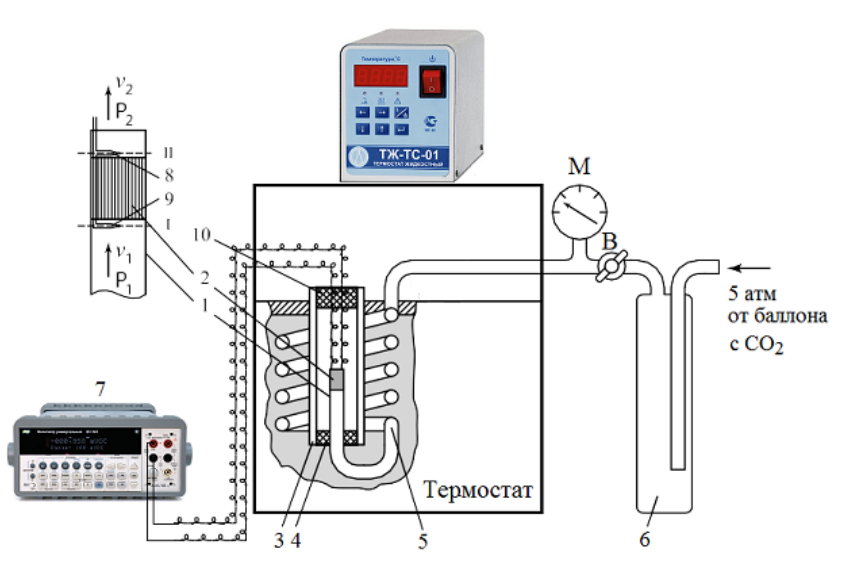
\includegraphics[width=15cm,height=10cm]{установка.png}
    \caption{Экспериментальная установка для исследования эффектов Джоуля-Томсона}
\end{figure}

\indent
Через турбку 1,сделанной из стали и потому обладающей малой теплопроводностью и
содержащей на конеце пористую перегородку 2, пропускается исследуемый
газ - двуокись углерода $CO_2$. Углекислый газ под повышенным давлением
попадает в трубку через змеевик 5 из баллона 6. Змеевик в свое время
медленно нагревает проходящий через него газ до температуры воды в термостате,
который поддерживает ее постоянной с точностью $\pm 0.1^{\circ}C$.
Манометр М измеряет разность давлений внутри трубки и снаружи.
Разность температур газа до и после перегородки измеряется дифференциальной
термопарой медь-констант, концы которой подключены к вольтметру. Если концы
термопары имеют разную температуру, то в цепи возникает разность потенциалов,
которая и измеряется вольтметром.

\section*{Экспериментальные данные}
\begin{table}[h!]
    \centering
    \begin{tabular}{|c|c|c|c|}
    \hline
    $\sigma_{\text{ман}}$, Бар & $max_{\text{ман}}$, Бар & $\Delta V$, мкВ & $C_{\text{P}}$, кДж/(кг$\cdot$К) \\\hline
    0.1 & 6 & 1 & 0.846 \\\hline
    \end{tabular}
    \caption{Некоторые константы и погрешности приборов}
\end{table}
\indent

\begin{table}[h!]
    \centering
    \begin{tabular}{|c|c|c|c|c|c|c|}
    \hline
        № & 1 & 2 & 3 & 4 & 5 & 6 \\\hline
        $\Delta P$, Бар  & 4 & 3.5 & 3.0 & 2.5 & 2.0 & 1.5 \\\hline
        $\Delta T^\circ C (T = 23.3^\circ C)$ & -3.87 & -3.28 & -2.71 & -2.22 & -1.66 & -1.29 \\\hline
        $\Delta T^\circ C, (T = 30^\circ C)$ & -3.71 & -3.13 & -2.71 & -2.13 & -1.55 & -0.97 \\\hline 
        $\Delta T^\circ C, (T = 40^\circ C)$ & -3.28 & -2.61 & -2.14 & -1.61 & -1.11 & -0.82\\\hline 
        $\Delta T^\circ C, (T = 50^\circ C)$ & -2.56 & -1.93 & -1.46 & -1.06 & -0.71 & -0.48\\\hline
    \end{tabular}
    \caption{Зависимость $\Delta P(\Delta T)$ при различных значениях $T$}
\end{table}

\indent
По полученным данным были построены графики зависимости $\Delta P(\Delta T)$ и 
по ним вычислены значения $\mu_{\text{д-т}} = \frac{\Delta P}{\Delta T}$ для 
разных температур. Результаты и сравнение с табличными данными приведины ниже.\\ 

\begin{table}[h!]
    \centering
    \begin{tabular}{|c|c|c|c|c|}
        \hline
        $T^{\circ} C$ & 23 & 30 & 40 & 50\\\hline 
        |$\mu_{\text{д-т}}$|, K/бар (экс) & 1.043 & 1.048 & 0.9901 & 0.8251\\\hline
        $\mu_{\text{д-т}}$, K/бар (табл) & 1.105 & 1.03 & 0.958 & 0.898\\\hline 
    \end{tabular}
    \caption{Сравнение экспериментальных и табличных значений коэффициентов Джоуля-Томсона}
\end{table}
Погрешность рассчитывалась по формуле:
\begin{align}
    \sigma_{\text{P}} = 0.1 \text{ бар; } \sigma_{\text{V}} = 0.003 \text{ мВ}\\ 
    \varepsilon_{\mu} = \sqrt{\left (\frac{\sigma_{T}}{T}\right )^2 + \left (\frac{\sigma_{P}}{P}\right )^2}\text{ ; }\varepsilon_{\text{max}}=7.7\%
\end{align}

\begin{figure}
    \centering
    \begin{subfigure}{0.45\linewidth}
        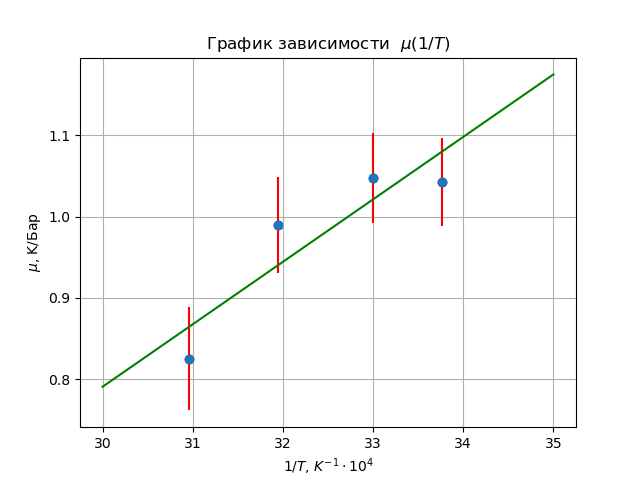
\includegraphics[width=8cm]{muT.png}
        \caption{График зависимости $\mu_{\text{д-т}}(\frac{1}{T})$}
    \end{subfigure}
    \hfill
    \begin{subfigure}{0.45\linewidth}
        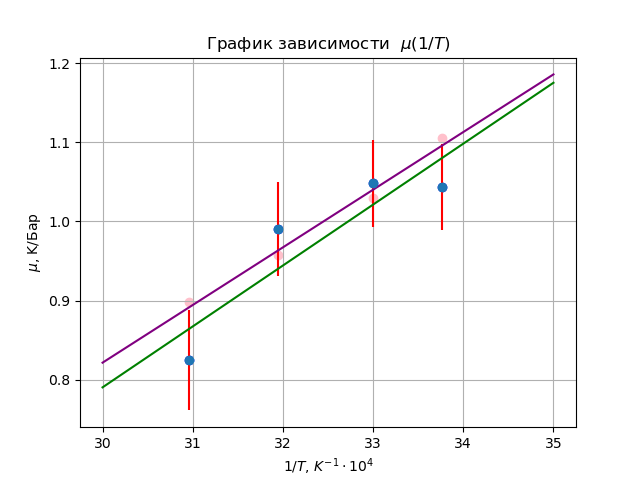
\includegraphics[width=8cm]{TableVal.png}
        \caption{Сравнение табличных и экспериментальных значений $\mu_{\text{д-т}}$}
    \end{subfigure}
\end{figure}

\begin{figure}
    \centering
    \begin{subfigure}{0.45\linewidth}
        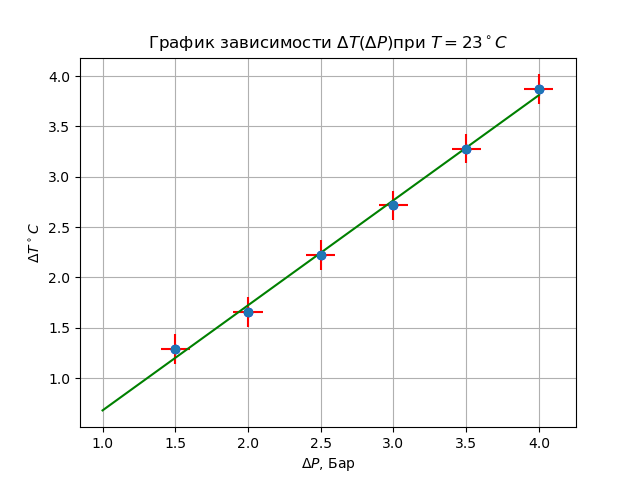
\includegraphics[width=8cm]{plot1.png}
        \caption{$\Delta P(\Delta T)$ при $T = 23.3^\circ C$}
    \end{subfigure}
    %\hfill
    \begin{subfigure}{0.45\linewidth}
        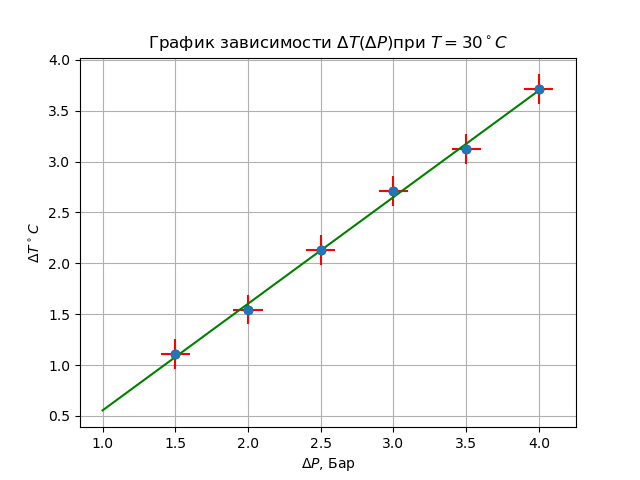
\includegraphics[width=8cm]{plot2.png} 
        \caption{$\Delta P(\Delta T)$ при $T = 30^\circ C$}
    \end{subfigure}
    \vfill
    \begin{subfigure}{0.45\linewidth}
        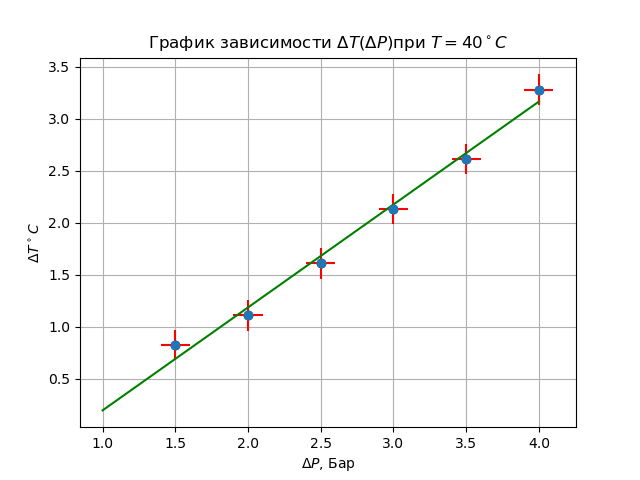
\includegraphics[width=8cm]{plot3.png} 
        \caption{$\Delta P(\Delta T)$ при $T = 40^\circ C$}
    \end{subfigure}
    %\hfill
    \begin{subfigure}{0.45\linewidth}
        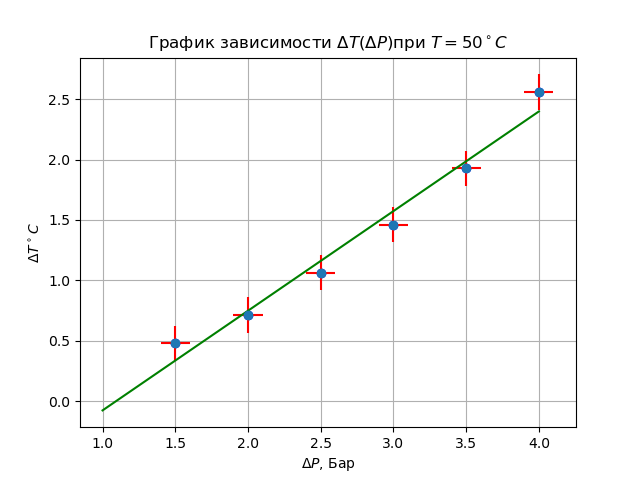
\includegraphics[width=8cm]{plot4.png} 
        \caption{$\Delta P(\Delta T)$ при $T = 50^\circ C$}
    \end{subfigure}
\end{figure}

\indent
Вычисляя по формулам $a, b, T_{\text{инв}}$ получаем:

\begin{align}
    a &= \frac{1}{2} \mu C_{p} R T = 0.0270 \pm 0.004 \text{ H$\cdot$м$^4$/моль$^2$; }a_{\text{табл}} = 0.36 \text{ H$\cdot$м$^4$/моль$^2$}\\[10pt]
    b &= \mu C_{p} = 12.8 \pm 0.9\text{ см$^3$/моль; }b_{\text{табл}} = 42.7 \text{ см$^3$/моль}\\[10pt]
    T_{\text{инв}} &= \frac{2a}{Rb} = 507 \pm 85\text{ К; }T_{\text{табл}} = 1520 \text{ К}
\end{align}

\section*{Результаты и выводы}



\end{document}
